% !TeX root = ../SPL-Rules.tex
% !TeX spellcheck = en_US
\section{Game Process}
\label{sec:game_process}

\subsection{Structure of the Game}
\label{sec:game_struct}

A game consists of four parts, pre-game meeting (see~\cref{sec:referee_team_communication}), the first half, a half-time break, and the second half.
Each half is \qty{10}{\minute} counted from the initial kick-off.
The half-time break is \qty{10}{\minute}, and during this time both teams may change robots, change programs, or do anything else that can be done within the time allotted.

The head referee signals the commencement of each half with a single whistle blow (that is, the Initial kick-off, \cf \cref{sec:initial-kick-off}).
The head referee signals the end of the first half with two short whistle blows, and the end of the second half with two short plus one long whistle blow.
The head referee should make \textit{all} of these whistle sounds from the T-junction of the halfway line.

\subsection{Robot States}
\label{sec:robot_states}

Robots can be in \textit{nine} different \emph{primary} states (see~\cref{fig:robot_states}).
Wireless connection must be available, so these states will be set by the GameController.
Teams must implement code to receive and correctly respond to wireless GameController packets, and also give a visual indication of the game state.

\textbf{The usage of the button interface as a replacement for any GameController commands/transitions is not allowed in the main competition!}

Should, on both teams, at least two robots have problems with the wireless network or GameController connection the head referee should issue a referee timeout (see \cref{sec:referee_timeout}).
If fewer robots do not respond to the GameController then they are, at the beginning, not included in the game (via a `Request for Pick-up', see \cref{sec:request_for_pickup}), and the game starts without the offending robot. The same applies to robots that no longer respond to the GameController at a later point in the game. Not responding means in this case that they are failing to react to the next GameController signal, such as a penalty or a change in game state.

The primary states are:
\begin{description}
  \item[Unstiff.] It helps to facilitate a consistent and safe handling of the robots for remote competition.
    During any state, if all head buttons are pressed at least one second, the robot should move to a safe seated/crouched position and unstiffen all joints.
    So while in the \texttt{unstiff} state the robot is not allowed to move in any fashion! After booting, the robots are in their \texttt{unstiff} state.
    Pressing the chest button once while in the \texttt{unstiff} state, permits the robot to stiffen its joints and return to the \texttt{initial} state, or a state as indicated by GameController.

    \item[Initial.] The robots are free to move at teams convenience and humans are allowed to interact with the robots. 
    This state is not limited in time and teams have access to the field.
    The GameController will activate this state before \texttt{standby} (i.e at the beginning of a half and during a timeout).
    Shortly pressing the chest button will switch the robot to the \texttt{penalized} state.

    \item[Standby.] The robots are not allowed to move in any fashion besides initially standing up and moving their heads.
    In \texttt{standby}, the robots are awaiting a visual indication from the referee which signals the transition to \texttt{ready}. 
    This state is used for Champions Cup matches only. For Challenge Shield matches, this state is skipped, and it is transitioned directly to \texttt{ready}. 

  \item[Ready.] In this state, the robots walk to their legal positions for kick-off (\cf \cref{sec:kick-off}) or a penalty kick (\cf \cref{sec:penalty_kick}).
    They remain in this state, until the head referee decides that there is no significant progress, up to a maximum of \qty{\KickOffAutoTime}{\second} for a kick-off and \qty{\PenaltyKickSetupTime}{\second} for a penalty kick.
    The GameController can activate sub-states for kick-off and penalty kicks.

  \item[Set.] In this state, the robots stop and wait for kick-off (\cf \cref{sec:kick-off}) or a penalty kick (\cf \cref{sec:penalty_kick}).
    Illegally positioned robots are \texttt{penalized} and placed on the side of the field.
    Robots are allowed to move their heads and arms or get up if fallen before the game (re)starts, but they are not otherwise allowed to move their legs or locomote in any fashion.
    If a robot cannot get up, fallen robot is called~(\cf \cref{sec:fallenrobots}).
    The penalty time counter is frozen during this state.
    Note that all penalized robots are left in place (on the side of the field, or in-place for motion in set) and must wait to get unpenalized.
    The GameController can activate sub-states for kick-off and penalty kicks.

  \item[Playing.] In the \texttt{playing} state, the robots are playing soccer.
    Shortly pressing the chest button will switch the robot to the \texttt{penalized} state.
    During the \texttt{playing} state, the GameController can activate the sub-states for free kicks (\cf \cref{sec:free_kick}).

  \item[Penalized.] A robot is in this state when it has been \texttt{penalized}.
    The only allowed movement is standing up after falling.
    Any other movement (including turning the head) is disallowed.
    Shortly pressing the chest button will switch the robot back to the \texttt{playing} state.

  \item[Finished.] This state is reached when a half is finished.

  \item[Calibration.] This state denotes the robot is acting with automatic calibration.
    This state may only be entered from \texttt{initial} by first pressing the front head button concluded by the chest button, for at least one second.
\end{description}

\begin{figure}[t]
  \centerline{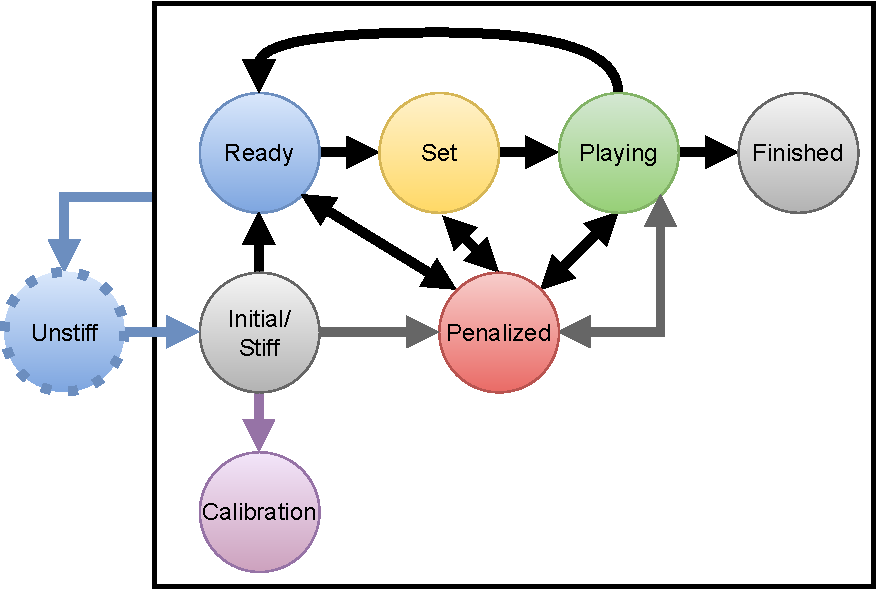
\includegraphics[width=0.9\columnwidth]{figs/states_new.pdf}}
  \caption{Diagram of the robot states.
    \\\textbf{Chest button} transitions are shown as gray arrows.
    However, any transition possible should be sent by the GameController.
    \\\textbf{GameController} transitions are shown as black arrows.
    \\Calibration transitions are shown as purple arrows which mean pressing the \textbf{front head button + the chest button}.
    \\From any state it can be transitioned to the \texttt{unstiff} state, shown as a blue arrow, via pressing all \textbf{three head buttons}.
    Pressing the \textbf{chest button} in the \texttt{unstiff} state allows a transition to the \texttt{initial} state, or a state as indicated by the GameController.}
  \label{fig:robot_states}
\end{figure}

At the scheduled time, the referee will announce that the transition from the \texttt{initial} to \texttt{standby} will be executed 60 seconds later.
The referee shall call ``Standby in 60 seconds''
The GameController operator will announce the transition from \texttt{initial} to \texttt{standby} when the head referee is calling ``Standby''.
If all humans from playing teams have left the field, the head referee can announce the transition earlier.


Once the game controller operator has confirmed the \texttt{standby} state, the referee should wait a random time between 10 to 120 seconds before announcing the transition to \texttt{ready}. 
Teams should expect that the delay before the referee signals the transition from \texttt{standby} to \texttt{ready} will be different every time.
To announce the transition from \texttt{standby} to \texttt{ready} state, the referee will raise both hands over their head.
Red gloves will be worn by the referee, though teams are encouraged not to rely on this visual cue as the gloves could be removed in a following year.
The referee must stand on the opposite side of the technical area behind the touchline and in line with the halfway line.
The signal must be held for \qty{\VisualSignalTime}{\second}.
The GameController signal for the transition from \texttt{standby} to \texttt{ready} will be delayed by \qty{\SetDelayTimeChampion}{\second} for Champions Cup and by \qty{\SetDelayTimeChallenge}{\second} for Challenge Shield.


The referee will announce the start of the \texttt{playing} state with a single whistle blow.
The GameController \texttt{playing} signal will be delayed by \qty{\PlayingDelayTime}{\second}.
This delay applies to both kick-off and penalty kicks.

The current game state should be displayed on the LED in the torso.
The colors corresponding to the game states are:
\begin{itemize}
  \item \texttt{Unstiff}: Blue-Blinking
  \item \texttt{Initial}: Off
  \item \texttt{Standby}: Cyan
  \item \texttt{Ready}: Blue
  \item \texttt{Set}: Yellow
  \item \texttt{Playing}: Green
  \item \texttt{Penalized}: Red
  \item \texttt{Finished}: Off
  \item \texttt{Calibration}: Purple
\end{itemize}

The current GameController requires robots to know both their team number and their robot number within the team.
It is each team's responsibility to make sure this is correctly configured.
It is recommended that the robot indicates its number within the team on boot up so that this can be easily checked at the start of the game.

\subsection{Goal}
\label{sec:goal}

A goal, including own goal, is achieved when the entire ball (not only the center of the ball) goes over the goal-side edge of the goal line, \ie the ball is completely inside the goal.\footnote{
  The goal line is part of the field.
}

The head referee signals a goal by a single whistle blow, followed by the call ``Goal \textless color\textgreater''.
The head referee should point with one arm towards the center of the field.
To assist robots listening for whistles, the referee should blow the whistle from on the carpet at the end of the fields where the goal was scored.

After a team scores a goal, the game proceeds with a kick-off (\cf~\cref{sec:kick-off}) for their opponents.
The GameController signal (to the robots) of a goal being scored, will be delayed by \qty{\GoalScoredDelay}{\second}.

\subsubsection{Invalid Goal}
\label{sec:invalid_goal}

A goal is invalid (that is, it can never be awarded) in the following circumstances:
\begin{enumerate}
    \item When an indirect kick is required but has not occurred (see~\cref{sec:indirect_kick_default}).
    \item When the last contact of the ball was with an attacking robot that played the ball with the arms/hands as defined in \cref{sec:hand_ball}.
      However, an own goal may be scored by any defending robot playing with arms/hands.
    \item When a team scores on themselves and there are no opponent robots on the field that are active (a definition of \emph{active} is given in \cref{sec:fallenrobots}).
\end{enumerate}

In these cases a goal is not scored (that is, the goal is ruled invalid), and the game will proceed with a Goal Kick (\cf \cref{sec:free_kick}).
The head referee should also advise why the goal is invalid, such as by calling ``Not indirect'', ``Played with hands'' or ``No own goal''.

\subsection{Indirect Kick}
\label{sec:indirect_kick_default}

\textbf{In Champions Cup and Challenge Shield,} both teams may only score a goal through two distinct ball contacts involving different robots within its own team following any affected start or restart in the \texttt{playing} phase, regardless of the initiator of the set play/free kick:

\begin{itemize}
  \item A robot may not score a goal from a direct kick, including via deflections.
  \item Set plays considered to be indirect are \texttt{Kick-off}, \texttt{Kick-in}, \texttt{Pushing free kick}, \texttt{Corner kick} and \texttt{Goal kick} or after an unsuccessful \texttt{Penalty kick}.
  \item The ball must be deliberately played-at a second time by another robot of its own team before a goal may be scored.
    A deliberate play at the ball includes successfully kicking the ball, dribbling the ball or the goalkeeper playing at the ball with its hands.
  \item If an indirect free kick is kicked directly into the opponent's goal, the goal does not count and a \texttt{Goal kick} is awarded.
  \item Note that an own-goal may always be scored without requiring an indirect kick.
\end{itemize}

There are two exceptions to this rule:

\begin{itemize}
  \item A direct kick is allowed for the duration of the penalty kick, but this rule still applies after this kick.
  \item If a team is awarded a free kick but fails to execute it within the allotted time, the opposing team may attempt to score directly if they play the ball before the team who was originally awarded the free kick does.
    ("Execute" is intended as "kick and move the ball clearly", as per section \cref{sec:free_kick_execution})
\end{itemize}

In both cases, the direct goal is only allowed if the kicking robot played the ball once.
\unsure{Updated after discussion, but not closed yet}
The indirect kick rule returns into effect when the ball comes to a full stop after the kick, or if the same robot plays the ball again before then.
In this case, any contacts made by the kicking robot, or any other robot, during the direct kick count towards the indirect kick rule.

\begin{description}
  \item[Example 1:] Player 2 (of the red team) kicks the ball to Player~3 (of the red team), who then kicks the ball into the blue team's goal.
  This is a successful indirect kick, and the goal counts.
  \item[Example 2:] Player 2 (of the red team) kicks the ball at the goal, and it is deflected off the side of the foot of a blue-team robot into the goal.
    This is \textit{not} an indirect kick, the goal does not count and a \texttt{Goal kick} is awarded to the blue team.
  \item[Example 3:] Player 2 (of the red team) kicks the ball ``upfield''.
    A blue-team robot kicks the ball a short distance, after which Player~2 kicks the ball again into the blue team's goal.
    This is \textit{not} an indirect kick, the goal does not count and a \texttt{Goal kick} is awarded to the blue team.
  \item[Example 4:] Player 2 (of the red team), walks up to and dribbles the ball.
    Player~2 then stop, and visibly back away from the ball, before approaching to dribble a \textit{second} time. The robot then scores.
    This is \textit{not} an indirect kick, the goal does not count and a \texttt{Goal kick} is awarded to the blue team.
  \item[Example 5:] Player 2 (of the red team) kicks the ball ``upfield''.
  A blue-team robot kicks the ball again into the red team's goal.
  This is \textit{not} an indirect kick, the goal does not count and a \texttt{Goal kick} is awarded to the red team.
  \item[Example 6:] Player 2 (of the red team) is awarded a \texttt{Penalty kick} and kicks the ball towards the blue-team's goal. The goalkeeper blocks the ball. The referee then calls ``Ball Free``.
  Player 2 (of the red team) kicks the ball again and score.
  This is \textit{not} an indirect kick, the goal does not count and a \texttt{Goal kick} is awarded to the blue team.
  \item[Example 7:] The blue team is awarded a free kick, but doesn't play the ball. The timer expires, and Player 2 (of the red team) kicks directly into the blue goal.
  The failed-free-kick exception applies, and the goal counts.
  \item[Example 8:] The blue team is awarded a free kick, but doesn't play the ball. The timer expires, and Player 2 (of the red team) kicks the ball 1 meter away.
  The ball stops, Player 2 kicks again, and scores.
  The exception does \textit{not} apply for the red team because Player 2 played the ball twice. The goal does not count and a \texttt{Goal kick} is awarded to the blue team.
  \item[Example 9:] The blue team is awarded a free kick, but doesn't play the ball. The timer expires, and Player 2 (of the red team) passes the ball to Player 3 (of the red team), who kicks again and scores.
  Although the exception doesn't apply because Player 3 played the ball as well, this is still an ordinary indirect kick, so the goal counts.
  \item[Example 10:] The blue team is awarded a free kick, but doesn't play the ball. The timer expires, and Player 2 (of the red team) kicks the ball 1 meter away.
  Player 5 (of the blue team) kicks the ball, then Player 2 kicks and scores.
  The exception does \textit{not} apply for the red team because Player 5 also played the ball. The goal does not count and a \texttt{Goal kick} is awarded to the blue team.
  \item[Example 11:] The blue team is awarded a free kick, but doesn't play the ball. The timer expires, then Player 5 (of the blue team) kicks the ball.
  Player 2 (of the red team) then kicks the ball and scores.
  The exception does \textit{not} apply for the red team because a blue-team robot played the ball first. The goal does not count and a \texttt{Goal kick} is awarded to the blue team.
\end{description}

\subsubsection{Fallback mode for Challenge Shield}

This rule aims to allow \textbf{Challenge Shield} teams to play games
even in the unfortunate case where severe circumstances make them unable to
field enough robots to play by the default indirect kick rules.

Each Challenge Shield team participating in a game shall declare their operational
capacity for that game by choosing to play either in \textbf{normal mode} or in \textbf{fallback mode}.
If at least one team plays in \textit{fallback mode}, the whole game follows different,
more lenient rules for indirect kicks, detailed in \cref{sec:indirect_kick_old}.

If a team plays in \textit{fallback mode}, they are only allowed to field at most two robots.
The other robots must be removed from the field via \texttt{Request for Pickup}.

Teams decide which operational mode to play in before the beginning of each half.
Furthermore, during any timeout (regardless of who initiated it), each team
may choose to switch from \textit{normal mode} to \textit{fallback mode}, but not vice versa.
In both cases, teams must inform the head referee and the GameController operator
of their choice, and they are encouraged to make this decision as early as possible.
% TODO maybe "2 minutes before the scheduled start/resume of the game"?

Changing operational modes during normal gameplay is not allowed.

\info[inline]{
  Besides preventing strategic abuses of the rule, having so few opportunities to change operational mode
  is also intended to help referees, ensuring that the indirect kick rules don't
  suddenly change during normal gameplay.
}

The GameController communicates to the robots the operational mode each team plays in,
while the TeamCommunicationMonitor and the GameStateVisualizer display this
same information for the convenience of the referees.

\subsubsection{Indirect Kick in fallback mode}
\label{sec:indirect_kick_old}

As long as at least one team plays in \textit{fallback mode}, \textbf{both teams}
play by the following rules instead of the default ones for indirect kicks.
\todo[linecolor=gray,backgroundcolor=gray!25,bordercolor=gray]{
  Remove the footnote after RC2025 has passed
}
\footnote{For reference, teams who participated in Challenge Shield in 2024 may notice that these are the same indirect kick rules used that year. They have been slightly rephrased to fit their new role, but they are functionally unchanged.}

Under these variant rules, after any restart into \texttt{playing} from a free kick,
the attacking team may only score a goal via an indirect kick.
Set plays considered to be indirect are \texttt{Kick-in}, \texttt{Pushing free kick},
\texttt{Corner kick} and \texttt{Goal kick} or after an unsuccessful \texttt{Penalty kick}.

The conditions for an indirect kick to be valid while at least one team
plays in \textit{fallback mode} are as follows:

\begin{itemize}
  \item A robot may not score a goal from a direct kick, including via deflections.
  \item The ball must be deliberately played-at a second time (by either another robot, or the same robot) before a goal may be scored.
    A deliberate play at the ball includes successfully kicking the ball, dribbling the ball (and subsequently leaving possession of the ball), or the goalkeeper playing at the ball with its hands.
  \item If a robot plays the ball to itself, this means that the ball must leave a circular area of at least \qty{0.75}{\metre} around the robot before the ball is played a second time and to be considered as an indirect kick.
\end{itemize}

Direct kicks are only allowed in the following situations:

\begin{itemize}
  \item On the first kick at \texttt{kick-off}.
  \item For the duration of a penalty kick, though the indirect kick rule returns into effect after the set play expires. In this case, any plays made during the penalty kick count towards this rule.
  \item Note that an own-goal may always be scored without requiring an indirect kick.
\end{itemize}

\begin{description}
  \item[Example 1:] Player 2 (of the red team) kicks the ball to Player~3, who then kicks the ball into the blue-team's goal.
    This is a successful variant indirect kick, and the goal counts.
  \item[Example 2:] Player 2 (of the red team) kicks the ball at the goal, and it is deflected of the side of the foot of a blue-team's robot into the goal.
    This is \textit{not} an indirect kick, and the goal does not count.
  \item[Example 3:] Player 2 (of the red team) kicks the ball ``upfield''.
    A blue-team robot kicks the ball a short distance, after which Player~2 kicks the ball again into the blue team's goal.
    This is a successful variant indirect kick, and the goal counts.
  \item[Example 4:] Player 2 (of the red team), walks up to and dribbles the ball.
    To be an indirect kick, Player~2 must then stop, and visibly back away from the ball, before approaching to dribble a \textit{second} time.
    The robot then scores.
    This is a successful variant indirect kick.
\end{description}

\subsection{Field-Side Selection and Initial Kick-off}
\label{sec:field_side_and_initial_kickoff}

\begin{itemize}
  \item The head referee throws a coin with one side for the home team and the other side for the away team according to the schedule.
    The team that wins the coin toss can either choose which goal to play for in the first half or take the kick-off.
  \item Depending on the decision above, the opposing team is given either the kick-off or may choose which goal to play for in the first half.
  \item The team that decided which goal to play for in the first half takes the kick-off at the start of the second half.
  \item In the half-time break both teams switch the sides of the field at play for the other goal.
  \item Teams must not change primary jersey colors for field players or goalkeepers during a match.
\end{itemize}

\subsection{Initial Kick-off}
\label{sec:initial-kick-off}

The first kick-off at the start of each half or after a timeout is an initial kick-off.
Robots have to be ready next to the field at latest \qty{2}{\min} before an initial kick-off.
All robots must be in the \texttt{unstiff} state.

Latest \qty{1}{\min} before the game starts all robots must be placed on the touchlines facing the other touchline in their own half by their team.
% (if present in person at the competition site) or their responsible referee according to \cref{fig:initial_positions}.
% If a team places robots themselves for initial kick-off, it is allowed for the team to vary the spacing and orientation of the robot positions along legal positions on their half's touchlines~(see also~\cref{sec:inside_outside}).

Robots are brought into the \texttt{initial} state after they are placed.
Once the robots receive the \texttt{ready} visual signal from the referee or the signal from the GameController, whichever happens first, they proceed as described in \cref{sec:kick-off}.

% \begin{figure}[t!]
%   \begin{center}
%     \leavevmode
%     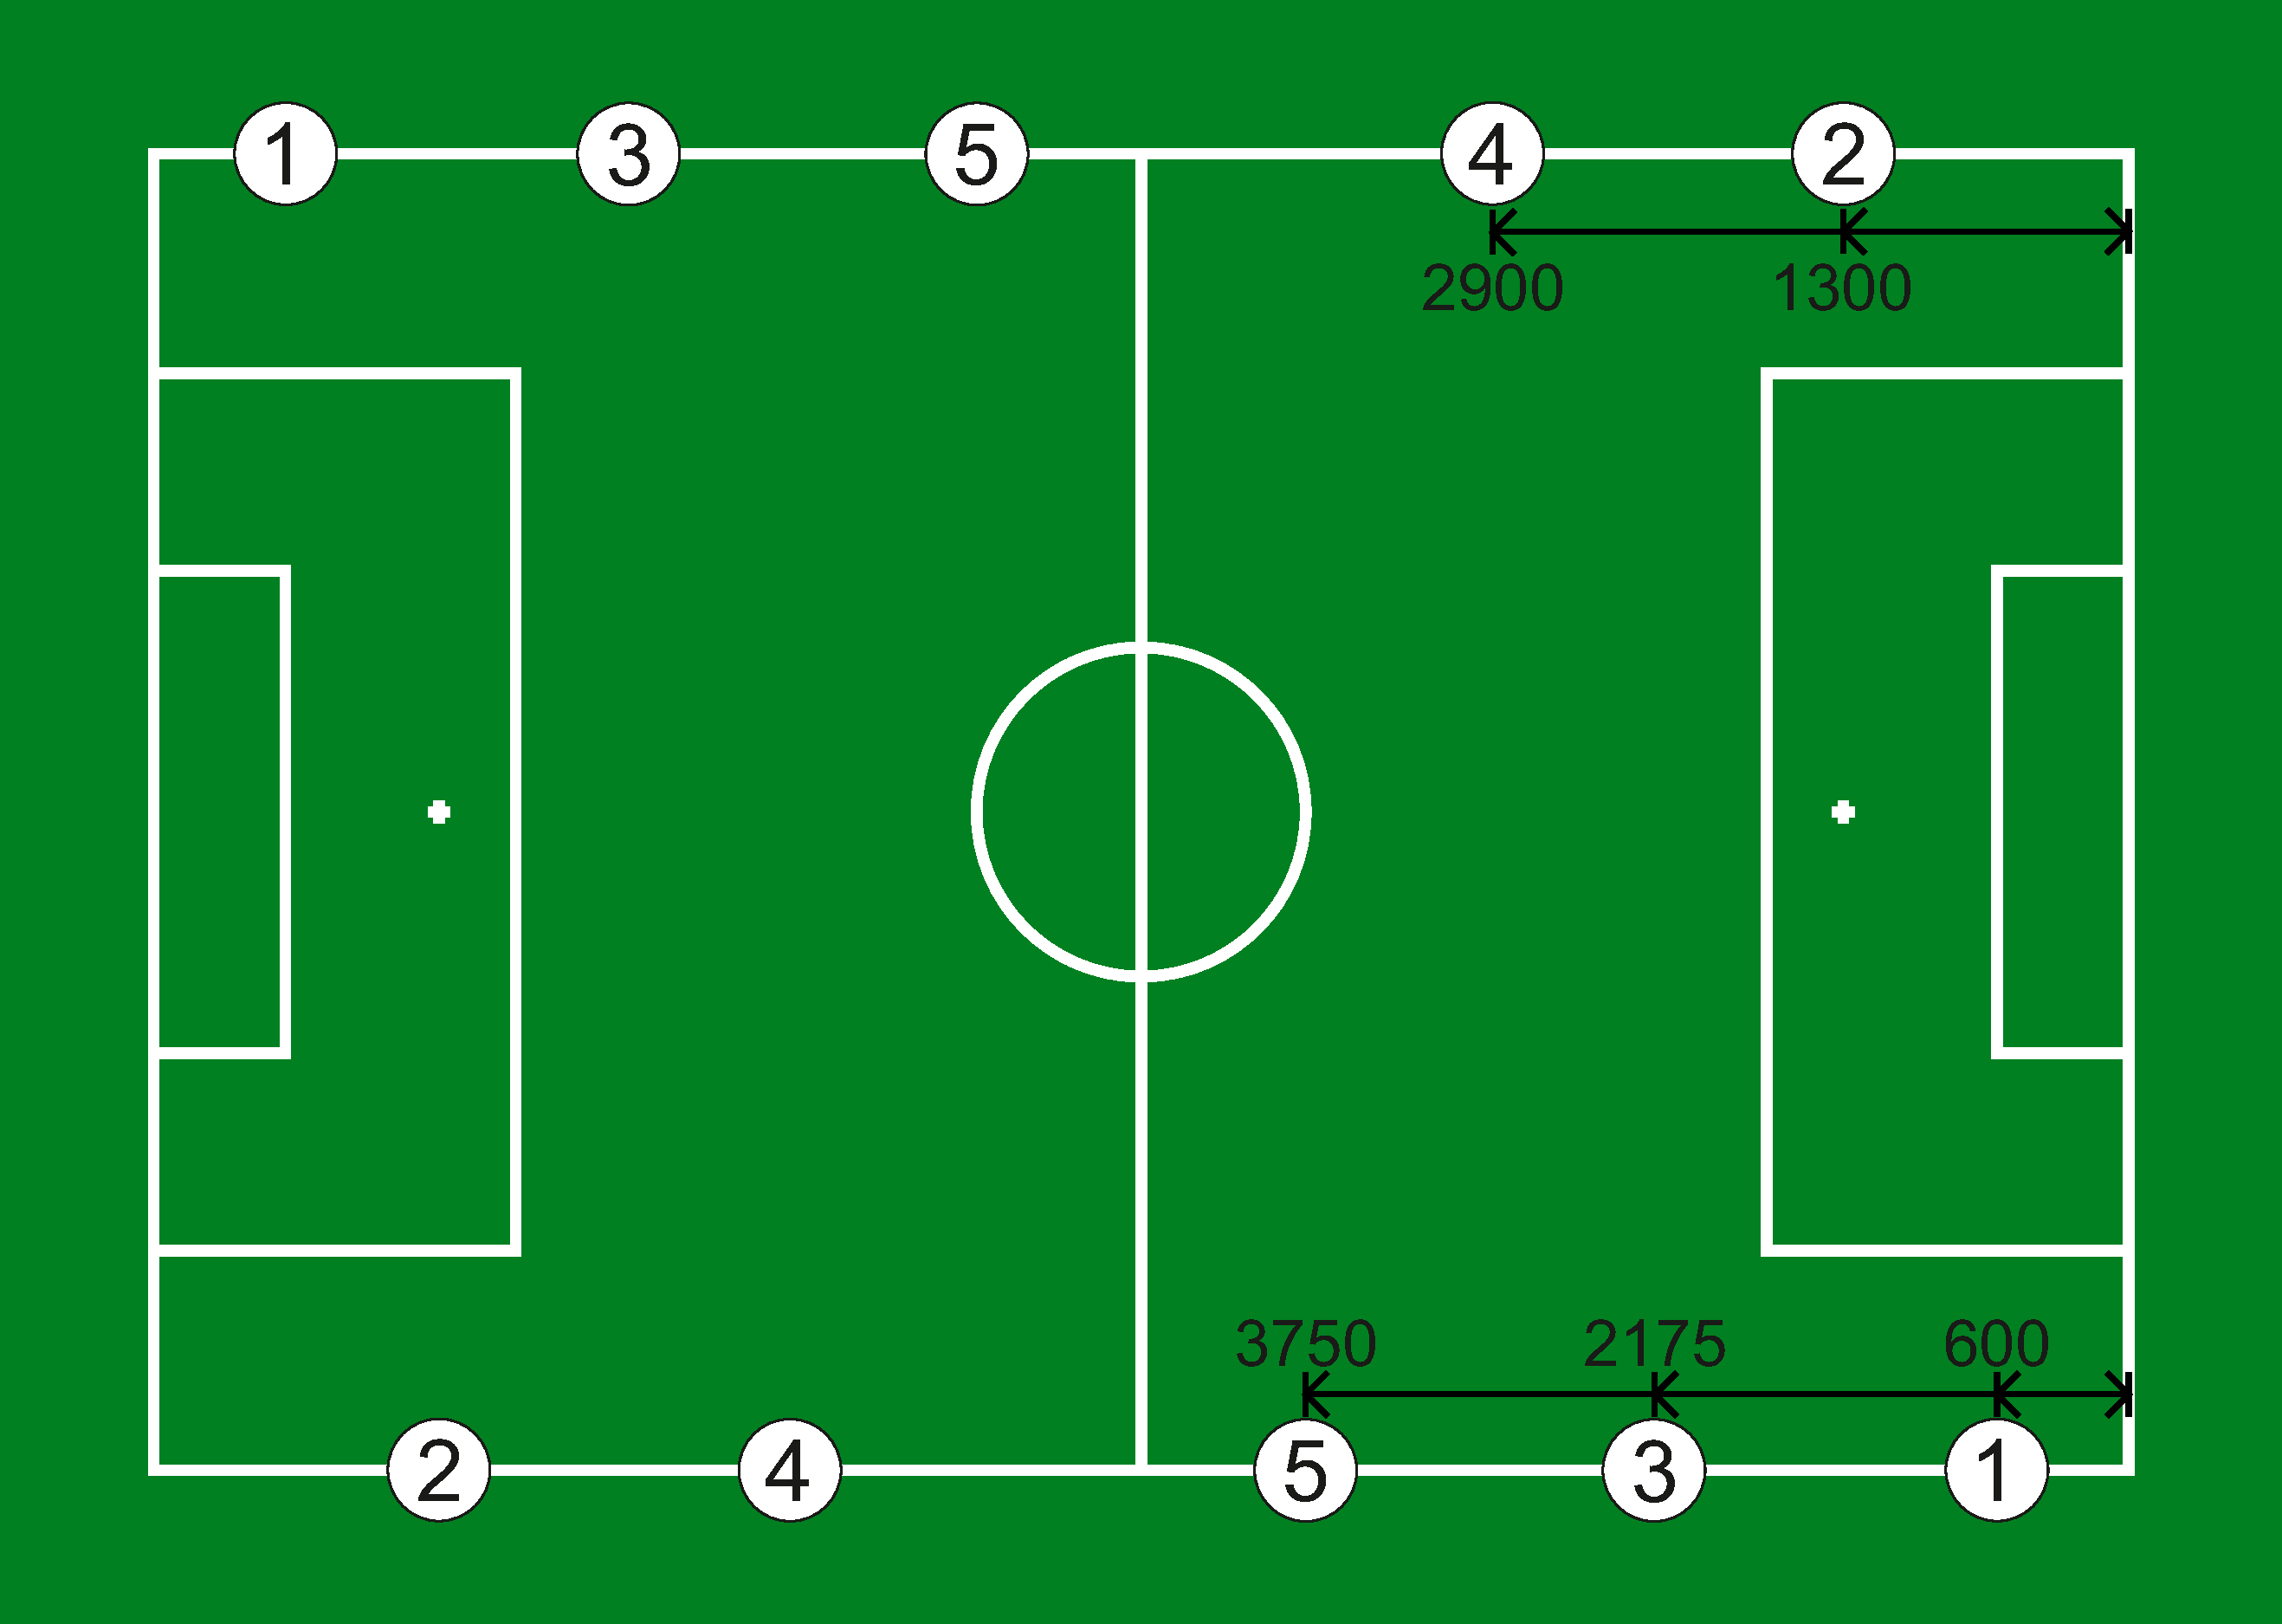
\includegraphics[width=1\columnwidth]{figs/initial_positions.pdf}
%     \caption{Positions, player numbers and distances from the center of the goal line for the initial kick-off of the robots.}
%     \label{fig:initial_positions}
%   \end{center}
% \end{figure}

\subsection{Kick-off}
\label{sec:kick-off}

For kick-off, the robots run through three states: \texttt{ready}, \texttt{set}, and \texttt{playing}.

In the \texttt{ready} state, the robots must walk to legal kick-off positions for their team.
Upon reaching the \texttt{set} state, the robots must stop and remain stationary until the kick-off is signaled by the referee (\cf~\cref{sec:motion_in_set}).
The following restrictions apply from the beginning of the \texttt{set} state until the ball comes into play:
\begin{itemize}
  \item The kick-off team can be positioned within their own half and the center circle.
    No robot may block the center mark.
    Up to one robot of the kick-off team is allowed to be outside the own half, provided it is inside the center circle.
    If more than one robot is outside the own half, only the one closest to the center mark is legal.
    This robot is then called \emph{kick-off} player and must execute the kick-off.
    If any other robot of the kick-off team executes the kick-off, the robot wrongly taking the kick-off is considered to be illegally positioned and a moved ball is placed back.
  \item The defending team can be positioned within their own half excluding the center circle.
  \item Robots are allowed to be positioned inside their own goal.
    All other positions that are fully on the border strip are illegal for both teams.
  \item Both teams are also subject to restrictions on the goal area (\cf~\cref{sec:ip_own_goal_area}).
\end{itemize}
All robots that do not reach legal positions before the \texttt{set} state begins or enter illegal positions before the ball is in play will be penalized with the ``Illegal Position'' penalty~(\cf \cref{sec:ip_kick_off}).
An exception applies to robots making reasonable effort to return to the field from a standard penalty and must not be penalized for illegal position.


A referee places the ball on the center mark.
If the ball is moved by one of the robots during the \texttt{set} state, it is placed back by one of the referees.

The head referee signals the kick-off by a single whistle blow, followed by the call ``Playing''.
The head referee must signal this from the T-junction of the halfway line.
\qty{\PlayingDelayTime}{\second} after the head referee has signaled the kick-off, the robots' state is switched to \texttt{playing} by the GameController (regardless of when the ball comes into play).

\subsubsection{Ball in Play}

The ball is in play and kick-off ends once
\begin{itemize}
  \item it is touched by the attacking team and moved clearly or
  \item \qty{\KickOffBallFreeTime}{\second} have elapsed in the \texttt{playing} state.
\end{itemize}

The GameController and head referee will indicate this by the call ``Ball Free''.

\subsection{Kick-in}
\label{sec:kick_in}

A ball is considered to have left the field when there is no part of the ball over the outside of the boundary line (\ie the line itself is in).
If the ball leaves the field it will be replaced on the field by an assistant referee.
Balls are deemed to be out based on the team that last touched the ball, irrespective of who actually kicked the ball.

If the ball goes over a touchline then the assistant referee will replace the ball back on the point of that touchline where it went out.
A free kick (\cf \cref{sec:free_kick}) is awarded to the team that did \emph{not} last touch the ball by the referee calling ``Kick-in \textless color\textgreater''.

If the ball goes over a goal line then the assistant referee will replace the ball back on the field, depending on which team last touched the ball.

\begin{itemize}
  \item If the ball was last touched by the defensive team, a \emph{Corner Kick} (\cf \cref{sec:free_kick}) is awarded to the attacking team.
    The referee calls ``Corner Kick \textless color\textgreater'' and the ball is placed on the corner on the same side of the field that the ball was kicked-out.
  \item If the ball was last touched by the offensive team, a \emph{Goal Kick} (\cf \cref{sec:free_kick}) is awarded to the defensive team.
    The referee calls ``Goal Kick \textless color\textgreater'', and the ball is placed on the corner of the goal area on the same side of the field that the ball was kicked-out.
    That is, the corner inside the field, not the T-junction where the goal area meets the goal line.
\end{itemize}

In these examples, ``red half of the field'' refers to the half the red team is defending.

\textbf{Example 1:} The red goalkeeper kicks the ball out the end of the field to the right of the goal.
The referee calls ``Corner Kick blue'', the ball is placed on the corner to the right of the goal and a free kick is started.

\textbf{Example 2:} A blue robot kicks the ball out the end of the field to the right of the goal the red team is defending.
The referee calls ``Goal Kick red'' and the ball is placed on the right corner of the goal area.

\textbf{Example 3:} A blue robot at midfield kicks the ball over the left touchline \qty{2}{\metre} into the red half of the field.
The referee calls ``Kick-in red'' and the ball is replaced on the left touchline where it went out.

\textbf{Example 4:} A blue robot kicks the ball but the ball touches a red robot at midfield before leaving the field near the halfway line.
The ball is regarded as out by red, the referee calls ``Kick-in blue'' and the ball is replaced on the touchline where it went out.

\subsection{Free Kick}
\label{sec:free_kick}

A free kick is initiated:
\begin{itemize}
  \item When the ball goes over the touchlines, termed \emph{Kick-in}.
  \item When the ball goes over the goal lines initiated by the defensive team, termed \emph{Corner Kick}.
  \item In place of a goal line Kick-in initiated by the offensive team, also termed a \emph{Goal Kick}.
  \item When a pushing penalty (see \cref{sec:player_pushing}) is awarded near the ball, termed a \emph{Pushing Free Kick}.
\end{itemize}

The head referee will announce a free kick, calling one of:
\begin{enumerate}
  \item For a \textit{Kick-in/Goal Kick/Corner Kick}: ``Kick-in/Goal Kick/Corner Kick \textless team\textgreater'' for the team that did not last touch the ball.
  \item For a \textit{Pushing free kick}: ``Foul \textless offending color\textgreater \textless offending number\textgreater'' for the pushing robot.
\end{enumerate}

The GameController will then activate the sub-state for the respective free kick.
Note that in the case of the Pushing free kick the sub-state is activated automatically through the ``Foul''.
The team who is awarded the free kick (termed the attacking team) has \qty{\FreeKickTime}{\second} to complete the kick.

\subsubsection{Visual gesture}
\label{sec:free_kick_gesture}

\textbf{In Champions Cup only}, the referee communicates which team is to take the free kick via a visual gesture.
The GameController packet will tell the robots which free kick sub-state is active, but not who is to kick the ball.

\begin{figure*}[t]
  \centering
  \begin{subfigure}{.33\textwidth}
      \centering
      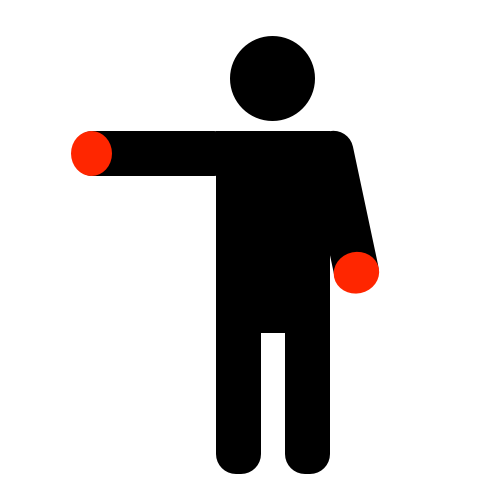
\includegraphics[height=120px]{figs/visual-signal/kick-in.png}
      \caption{Pointing to the left goal}
  \end{subfigure}
  \begin{subfigure}{.33\textwidth}
      \centering
      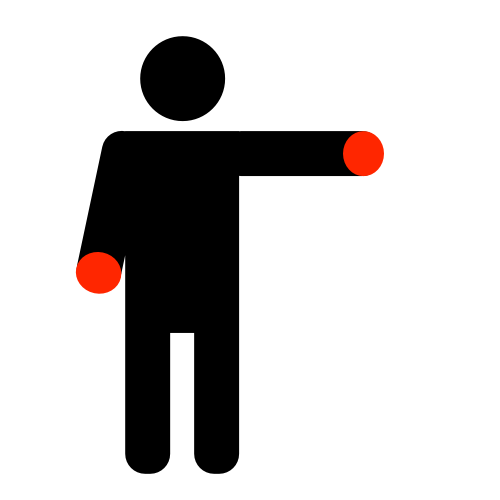
\includegraphics[height=120px]{figs/visual-signal/kick-in-flipped.png}
      \caption{Pointing to the right goal}
  \end{subfigure}
  \caption{Visual signals for set plays.}
\end{figure*}

The gesture consists of raising one arm horizontally and sideways, parallel to the field line, while the other arm remains at rest.
The raised arm is the one pointing towards the defending team's goal, i.e. the goal of the team that is \textit{not} taking the free kick.
\todo[linecolor=gray,backgroundcolor=gray!25,bordercolor=gray]{
  Remove the footnote after RC2025 has passed
}
\footnote{For reference, teams who participated in the 2023 Visual Referee Challenge
  may notice that this the same as the "Kick-in" gesture from back then,
  but with the opposite arm raised.
}

This gesture is made by the head referee and held for at least 5 seconds after the GameController signal is sent.
The head referee is encouraged to seek the acknowledgement of the GameController operator and/or look at the field-facing monitor (if available) in order to determine the timing.

The referee makes an effort to send the signal standing as close as possible to the T-junction joining the half-way line to the touchline opposite to the technical area.
However, their actual positioning along the touchline may deviate slightly from this standard position, based on the current game situation and the timing of the gesture.
\info[inline]{Remind the refs that the GC operator will take a few moments to click the button, giving them a little time to make a couple steps if needed.}

Teams are encouraged to make an effort to familiarize with looking at the referee and interpreting the visual signal even in cases where such an action may not seem strictly necessary,
as more information may be communicated in this way rather than via GameController packets in future years.

\textbf{In Challenge Shield}, this visual signal does not need to be performed and the kicking team is communicated by the GameController.
\info[inline]{In accordance with the teams, the referee may still perform the gesture if e.g. a team wants to experiment with recognition, without changing the GC behavior.}

\subsubsection{Execution}
\label{sec:free_kick_execution}

When necessary, the referee may need to place the ball.
For a pushing free kick, the ball will be left in place, and only repositioned in accordance with the pushing rules (see \cref{sec:player_pushing}).
If the ball left the field, the ball will be positioned as described in \cref{sec:kick_in}.

During the free kick, only the attacking team may approach within \qty{\FreeKickRadius}{\metre} to the ball.
All robots of the defensive team must immediately move away from the ball.
Defensive robots that violate these restrictions are penalized with the ``Illegal Positioning'' penalty (see \cref{sec:illegal_positioning}) which results in a standard removal penalty~(see \cref{sec:removal_penalty}).
Additional penalties against any further robots during the free kick, including Pushing, do not result in an additional free kick, but still use the appropriate removal penalty.

A free kick is deemed completed and play returns to normal if:
\begin{itemize}
  \item The attacking team moves the ball clearly, except for a robot getting up which is exempt from this rule.
  \item The \qty{\FreeKickTime}{\second} time period expires (or the game time expires).
\end{itemize}
The head referee will announce a free kick is completed by calling ``Ball Free'', and the GameController resumes the game state \texttt{playing}.
Note that the sub-state will be automatically left after the \qty{\FreeKickTime}{\second} time period expires.

\subsection{Penalty Kick}
\label{sec:penalty_kick}

A penalty kick is initiated when a pushing penalty (see \cref{sec:player_pushing}) is awarded near the ball against the defending team within their own penalty area.
The head referee will announce a penalty kick by calling ``Penalty Kick \textless offending color\textgreater \textless offending number\textgreater'' for the pushing robot.

When the GameController activates the penalty kick, the game changes to the \texttt{ready} state with \texttt{penalty kick} sub-state active.

This denotes that the robots are given time to set up and prepare for the penalty kick.
Similar to kick-off, the game clock is \textit{paused} during finals games only.
The referees should pick up the ball.

\textbf{In Champions Cup only}, the GameController does not communicate the identities of the attacking and defending team.
Instead, this information is communicated via the same visual gesture described in \cref{sec:free_kick_gesture} for free kicks.

Robots have \qty{\PenaltyKickSetupTime}{\second} to get into position for the penalty kick.
At the end of \qty{\PenaltyKickSetupTime}{\second}, the game changes to the \texttt{set} state with \texttt{penalty kick} sub-state active.
Similar to a kick-off, during the \texttt{set} state the robots are waiting for the penalty kick to commence.
Standard penalties apply.
Additionally, only the goalkeeper robot from the defending team may be within the penalty area.
The goalkeeper robot must either be touching the goal line or stay outside its own penalty area.
If the goalkeeper positioned itself inside the goal area but ahead of the goal line it is placed back by the referee during \texttt{set} state, so the center of its feet touches the center of the goal line.
The placement should happen perpendicular to the goal line without rotating the robot.
If this manual placement would lead to a position the robot collides with a goalpost, it is placed inside or outside the goalpost on the goal line, depending on which position is closer.
Only one robot from the attacking team may be within the penalty area, and it may not block the penalty mark.
Blocking the penalty mark is considered to be an illegal position.
All robots that do not reach legal positions will be penalized with the ``Illegal Positioning'' penalty~(\cf \cref{sec:illegal_positioning}).

The referee should also place the ball on the penalty mark during \texttt{set}.
The referee signals the penalty kick commences by blowing the whistle once, and calling ``Playing''.
The game switches to the \texttt{penalty kick} sub-state of the \texttt{playing} game state, and the game clock is resumed.
(Note that the GameController signal is delayed by \qty{\PlayingDelayTime}{\second} when switching from \texttt{set} to \texttt{penalty kick} sub-state).
The attacking team has \qty{\PenaltyKickTime}{\second} to complete the penalty kick.

During the penalty kick:
\begin{enumerate}
  \item The defensive goalkeeper robot must always be in contact with the goal line if it is inside the penalty area, and must remain on its feet.
    The goalkeeper is only permitted to ``dive'', and be off its feet after the attacking robot has touched the ball.
  \item The attacking robot may move freely.
  \item All robots must be within the field-of-play.
    That is, robots may not be outside the field lines, but within the field border.
  \item No other robots may enter the penalty area (\cf \cref{sec:illegal_positioning}).
  \item Additional penalties against any further robots, including pushing, do not result in an additional free
    kick, but still use the appropriate removal penalty.
\end{enumerate}

The attacking robot (taking the penalty kick) may only score a goal if it touches the ball once.
Once the attacking robot has touched the ball, it may not score a goal until another robot (from either team) touches the ball.
If this robot ``scores'', it results in a goal kick~(\cf \cref{sec:invalid_goal}).

The penalty kick is deemed completed if:
\begin{itemize}
  \item The attacking team touches the ball, even if the robot has fallen.
  \item The \qty{\PenaltyKickTime}{\second} time period expires (or the game time expires).
\end{itemize}

The head referee will announce a penalty kick is completed by calling ``Ball Free'', and the GameController resumes the game state \texttt{playing}.
Note that the sub-state will be automatically left (returning to the \texttt{playing} state) after the \qty{\PenaltyKickTime}{\second} time period expires.

Note that the restrictions on the attacking robot still apply after the penalty kick is complete.

\subsection{Game Stuck}
\label{sec:game_stuck}

In the event of no substantial change in the game state for \qty{\GameStuckTime}{\second}, this is considered a game stuck.
``Substantial change'' can consist of a robot seeing and moving towards the ball OR robots exploring the field (presumably in an attempt to find the ball).

The main referee has two options how to solve the game stuck and to reestablish the chance of progress in the game.
The intention of the game stuck rule is to achieve progress with as little intervention as possible, \ie the \emph{Local Game Stuck} rule will be preferred, but only if there is a chance that its application will result in progress in the game.

\subsubsection{Local Game Stuck}
\label{sec:game_stuck:local}

If one robot is preventing the game from proceeding---perhaps by circling the ball repeatedly without kicking the ball---it is recommended to improve progress by removing this one robot.
The head referee calls ``Local Game Stuck \textless robot\textgreater'' for this robot, which is penalized (\cf \cref{sec:pen_local_game_stuck}).

\subsubsection{Global Game Stuck}
\label{sec:game_stuck:global}

If no robots have made progress towards the ball or began to explore the field in \qty{\GameStuckTime}{\second} Global Game Stuck may be called.
The referee calls ``Global Game Stuck'' to announce the decision.

Once the referee calls Global Game Stuck, players enter the \texttt{ready} state, and a new kick-off is awarded.
For the first Global Game Stuck of a half, the kick-off is awarded to the team that did not have the initial kick-off of the half.
For any further Global Game Stuck calls of a half, kick-off is awarded to the team that did not receive kick-off in the previous Global Game Stuck call.
The GameController will display which team should be awarded kick-off following a Global Game Stuck call.

A global game stuck can only be called if at least one robot has touched the ball since the previous kick-off.

\subsection{Request for Pick-up}
\label{sec:request_for_pickup}

Either team may request that one of their players be picked up (called ``Request for Pick-up'').
In the \texttt{playing} or \texttt{ready} state, players may only be picked up for hardware failures.
In all other states, players may be picked up for any reason.

Every change (hardware or software) is allowed during a request for pick-up.
In particular, it is permitted to change batteries, fix mechanical problems, reboot the robots, and change configuration files.
It is also allowed to replace a broken robot by a substitute robot.
Substitute robots must wear the correct jersey color for their role (goalkeeper or field player).
It is discouraged to change the robot's control program, \textbf{but not forbidden}.

Any strategic ``Request for Pick-up'' is not allowed.
That is, gaining an advantage by removing the robot from the game.
In this case, the head referee will indicate when the robot is no longer affecting play and can be removed from the field by an assistant referee.

To prevent mistakes and confusion during games, only team captains (\cf \cref{sec:referee_team_communication}) should make a ``Request for Pick-up'', and only one designated person per team shall accept the robot from the referee, and hand it back after fixing the problem.
The returning robot may be returned following the normal replacement procedure once at least \qty{\StandardPenaltyTime}{\second} have elapsed since the robot was removed from play.
Note that this penalty does not follow the standard removal procedure, and hence does not count towards the incremental penalty count.
If the picked-up robot was penalized, the penalty time of the robot counts down with the game clock throughout the pick-up.

The robot should be returned to the assistant referees in the \texttt{penalized} state.
Note here, that the returning robot or the substitute robot will have to wait out any remaining penalty time of the picked up robot after the team handed their robot back to the assistant referees.

\subsection{Request for Timeout}
\label{sec:request_for_timeout}

Each team can call a \textbf{maximum of 1 timeout per game} with a total time of no more than \textbf{5 minutes}.
During this time, both teams may change robots, change programs, or anything else that can be done within the time allotted.
During normal game time, a team may call a timeout at any stoppage of play (after a goal, stuck game, before a half, etc.).
Alternatively, a team may call a timeout before a penalty shootout if they have not used their timeout yet (\cf \cref{sec:penalty_shoot-out}).

The timeout ends when the team that called the timeout says they are finished, at which time they must be ready to play.
The other team must be ready to play at the time the timeout runs out, or \textbf{2 minutes} after a prematurely called end of the timeout, whichever is earlier.
If the other team is not ready to play in time, it has to call a timeout of its own.

The clock stops during timeouts, even during the preliminaries, and is reset to the time when the current stoppage of play began.

After the completion of the timeout, the game resumes with a kick-off for the team which did not call the timeout.

If a team is not ready to play at the assigned time for a game, the referee will call the timeout for that team.
After the expiration of such a timeout, if the team is still not ready to play then the referee shall start the game with only one team on the field.
The team that was not ready can return its robots to the field as per the rules for ``Request for Pick-up''.
If both teams are not ready, the referee will call timeouts for both teams.
This ``double timeout'' expires after 10 minutes.

\subsection{Referee Timeout}
\label{sec:referee_timeout}

The head official may call a timeout at any stoppage of play if he or she deems it necessary.
A referee timeout should only be called in dire circumstances---one example might be when the power to the wireless router is down or no robot listens to the GameController.
However, when and whether to call a referee timeout is left up to the head referee.

Referees may call multiple timeouts during a game if needed.
Teams may do anything during these timeouts, but they must be ready to play \textbf{2 minutes} after the referee ends a timeout.
The referee should end the timeout once he or she believes the circumstance for which the timeout was called has been resolved.
In cases where the circumstance for which the timeout was called is not resolved within 10 minutes, the chair of the technical committee should be consulted regarding when/if play should continue.

The team who would have kicked off if the timeout had not been called shall kick-off when the game resumes.

\subsection{Extra Time}
\label{sec:extra_time}

The head official may decide to add time to the clock if a substantial delay (such as an enormous wireless delay) causes excessive game time to be lost.
The decision to add time to the clock should be made immediately after the incident.
The GameController operator should execute this addition of time using the GameController interface.

\subsection{Mercy Rule}
\label{sec:mercy_rule}

A game will conclude once the game score shows a goal difference of 10.
Ending the game is mandatory once a goal difference of 10 is reached.

\subsection{Penalty Kick Shoot-Out}
\label{sec:penalty_shoot-out}

A penalty kick shoot-out is used to determine the outcome of a tied game when an outcome is required (for example, when team progression is tied on all tie-break factors, during the promotion round, intermediate round, quarterfinals, semifinals, third place or final).

All penalty kicks are taken against the same goal.\footnote{
  Which goal to take for the shoot-out is decided in accordance with the teams, or otherwise by a coin toss.
}
The team listed first on the competition schedule will have the striker robot for the first penalty kick.
Subsequently, both teams take kicks alternately.
At all stages of the competition, the penalty kick shoot-out will consist of three penalty kicks per team.
A team that has scored the most goals at the conclusion of these will be declared the winner.
A winner can also be declared before the conclusion of the penalty shoot-out if a team can no longer win.
If the two teams remain tied after three penalty kicks, then a sudden death shoot-out will follow until a definite winner is found.

The penalty kick shoot-out starts immediately without changing any code after the second half ended.
No timeouts may be called during the penalty shoot-out.
However, a team may request a timeout before the penalty shoot-out starts if they have a timeout remaining for this game.
During the timeout code changes are allowed.

Before the penalty shoot-out begins, each team must hand over to referees up to 6 prepared robots that may participate in the penalty shoot-out.
No robots may be added once the penalty shoot-out starts.
Robots that will not participate in the shoot-out must not be on the wireless network and must stay outside of the field.
All participating robots must be wearing the correct jersey for their player and no duplicate numbers are permitted.

During the entire penalty kick shoot-out, the robots are controlled by the GameController and the referee's whistle.
A team cannot request the referees to press buttons on their robots, except for initially leaving the \texttt{unstiff} state.

\subsubsection{Penalty Kick}
\label{sec:pso_kick}

A penalty kick is carried out with one striker robot and one opposing goalkeeper.
The penalty kick commences with the \texttt{set} game state activated.
Before each penalty kick, both teams must select the robot to participate (as goalkeeper or striker) in the penalty kick.
The team leader communicates the selection to the head referee by privately handing the referee a card with their chosen number.
After both teams have selected their player, the GameController operator selects the requested striker and goalkeeper robots from the opposing teams and the GameController communicates that all non-selected robots are substitutes and should remain inactive.
The GameController indicates which team has the striker robot in the current penalty kick.

Referees place the ball, the striker, and goalkeeper robots.
The ball is placed on the penalty mark closest to the goal being defended.
The striker robot is positioned on the edge of the penalty area, facing the ball and the goal.
The goalkeeper is placed with its feet on the goal line and in the center of the goal.
Neither robot is permitted to locomote (move their legs) during the \texttt{set} state.
Movement of the robot's head and arms is allowed.

The head referee commences the penalty kick by blowing the whistle \textit{once}, and calling ``Playing''.
The GameController activates the penalty kick, switching to the \texttt{playing} game state.
Note that the \texttt{playing} signal is delayed~(\cf \cref{sec:robot_states}).

The time limit for the striker is \qty{\PenaltyShootoutKickTime}{\second} after the penalty kick starts.
A penalty kick is over when the ball has come to a full stop after the first contact by the striker robot.
The striker robot is not allowed to play the ball a second time after the ball has clearly moved, otherwise the penalty kick ends immediately as well.
A goal is awarded to the attacking team if a goal has been scored (\ie the ball has completely crossed the goal line) before the penalty kick is over.
Otherwise, the score is unchanged.

The goalkeeper robot must always be in contact with the goal line and must remain on its feet until the striker robot touches the ball.
The goalkeeper is only permitted to ``dive'' and be off its feet after the attacking robot has touched the ball.
If the goalkeeper violates these rules, then the penalty kick ends immediately and a goal will be awarded to the attacking team.

All rules such as ``Ball Holding'', ``Pushing'' and others are applied during the penalty kick.
A goalkeeper will not be penalized for inactivity during a penalty kick, provided its stiffness is on.
Other penalties are applied as usual.

\subsubsection{Sudden Death Shoot-Out}
\label{sec:sudden_death_shoot_out}

Teams take one additional penalty kick each, and the game decision will be made as follows:
\begin{itemize}
  \item Each kick is ranked in one of the following categories:
  \begin{enumerate}
    \item goal
    \item kick at the goal that is blocked by the goalkeeper
    \item kick that hits a goalpost
    \item kick that crosses the goal line next to the goalposts
    \item any other kick
    \item no kick
  \end{enumerate}
  \item If both teams' kicks rank in different categories, the team with the higher ranked kick wins.
  \item Otherwise, the sudden death is repeated.
  \item If after 3 sudden death penalty kicks there is still no winner, the referee will toss a coin to decide the game.
\end{itemize}
